\documentclass[10pt]{article}
\usepackage[margin=20mm]{geometry}
\usepackage{amsmath,graphicx,booktabs,longtable,url}
\usepackage[hidelinks]{hyperref}
\newcommand{\Pparams}{18,962}
\newcommand{\Dparams}{19,450}
\newcommand{\DevN}{319}
\newcommand{\NegN}{2689}
\newcommand{\SessionN}{13}
\newcommand{\MatchedN}{311}
\newcommand{\MatchedPoints}{2,756}
\newcommand{\AllPoints}{2,818}
\newcommand{\TrainN}{55,980}
\newcommand{\UsableTrainN}{55,915}
\newcommand{\CalN}{1,004}
\newcommand{\SelectionN}{1,031}
\newcommand{\HeldoutN}{1,985}
\newcommand{\Rmedian}{6.616}
\newcommand{\Pmedian}{5.905}
\newcommand{\Improve}{0.711}
\newcommand{\ImproveLow}{0.411}
\newcommand{\ImproveHigh}{1.174}
\newcommand{\RPCK}{63.733}
\newcommand{\PPCK}{67.341}
\newcommand{\PDdelta}{-0.525}
\newcommand{\PDlow}{-0.980}
\newcommand{\PDhigh}{-0.210}
\newcommand{\TranslationImprove}{7.439}
\newcommand{\Ptime}{13.661}
\newcommand{\Pfulltime}{15.352}
\newcommand{\Rtime}{9.733}
\newcommand{\Rfulltime}{11.217}
\newcommand{\PriorAbstract}{The P--prior median difference is 0.336 pixels (paired-session interval [0.063,0.585]). The interval favors the prior, not P. This is a fixed-budget development comparison.}
\newcommand{\PriorTrainingStatus}{All three matched-budget fits were completed; the learning curves are diagnostic, not a best-checkpoint selector.}
\newcommand{\ConfirmationAbstract}{Independent real-session confirmation is not yet available.}
\newcommand{\ConfirmationProtocol}{Independent confirmation is awaiting new data. The collection plan starts with 12 separate sessions and 15 prespecified frames per session, with at least 30 frames independently double annotated before blind adjudication. This is not a power guarantee. Predictions are hidden during annotation and the full panel must be frozen before evaluation. Existing FINAL-named manifests have unavailable membership and are not treated as independent observations.}
\newcommand{\ConclusionPrior}{The source-derived prior comparison quantifies a fixed-budget tradeoff, not converged-method superiority.}
\newcommand{\ConfirmationConclusion}{Independent real-session confirmation remains required.}
\newcommand{\RuntimePanelStatus}{The expanded panel was measured in the same session for all comparators.}

% Generated evidence status: not a manuscript acceptance/submission flag.
\newcommand{\DopeAbstractStatus}{For frozen DOPE on reused DEV, the conditional keypoint median is 12.585 pixels before refinement and 7.461 pixels for the mean of three P seed statistics; full-GT PCK10 is 19.872 and 36.775 percent, respectively. }
\newcommand{\DopeMainStatus}{For frozen DOPE on reused DEV, the conditional keypoint median is 12.585 pixels before refinement and 7.461 pixels for the mean of three P seed statistics; full-GT PCK10 is 19.872 and 36.775 percent, respectively. The tables retain missing predictions and unfavorable outcomes.}
\newcommand{\DopeConclusionStatus}{The DOPE measurements describe one additional fixed application; they do not establish arbitrary-backbone transfer, independent TEST generalization or stable physical T/R improvement.}

% Completed ResNet18 direct-estimator and frozen-refiner evidence, October 2026.
\newcommand{\ThirdEstimatorStatus}{The third application is a completed full-image, nine-landmark Simple-Baselines-derived ResNet18. Its frozen FULL estimator receives RGB and registered physical dimensions, and its primary transfer test adds the same image-feature local refiner without a second dimension input (P0). D0 is the matched direct-residual control. P5 and P5\_CONSTANT form a separate dimension-input extension. All real-image outcomes are reused-development evidence.}
\newcommand{\ResnetAbstractStatus}{For the third, dimension-conditioned ResNet18 estimator, the primary P0 refiner changes reused-DEV conditional median error from 8.001 to 7.143 pixels and full-denominator PCK10 from 54.68\% to 58.28\%; reconstructed-reference translation and canonical camera-facing-frame C2 rotation medians change from 11.007~cm/3.252~deg to 10.001~cm/3.018~deg.}
\newcommand{\ResnetMainStatus}{The ResNet18 FULL estimator and all twelve D0/P0/P5/P5\_CONSTANT head fits completed. P0 is the primary third-backbone transfer arm; it improves central 2D development error and PCK10, while its translation interval includes zero. P5 is reported only as a separate dimension-conditioned-head extension because P5--P5\_CONSTANT does not establish stable joint 2D/T/R improvement.}
\newcommand{\ResnetConclusionStatus}{A third frozen feature interface supports the primary P0 refinement result on reused DEV, but the separate P5--P5\_CONSTANT comparison does not establish a robust incremental benefit from dimensions or stable physical T/R improvement.}
\newcommand{\ResnetBaselineStatus}{The completed direct-estimator study trains CONSTANT, SHAPE and FULL arms for a fixed 10 epochs on 55,980 synthetic TRAIN images (34,990 updates and 559,800 exposures per arm). All share seed 42, ImageNet ResNet18 initialization, identical source order and photometric augmentation. FULL supplies normalized $\log W$, $\log D$, $\log H$, $\log(W/D)$ and $\log(H/\sqrt{WD})$ to a decoder FiLM block; SHAPE keeps only the two ratios and CONSTANT supplies zeros. Epoch 10 is fixed using no real-image selection.}

\title{Supplementary Material: Local Refinement with Frozen Estimator Applications}
\author{Internal draft for author review}
\date{October 2026}
\begin{document}\maketitle
\section{Status and reading guide}
Tables and figures copied from the original manuscript describe historical YOLO experiments only. The DOPE extension is identified separately below; its unmeasured values are never filled from that panel. This supplement preserves the distinction between completed development evidence and independent confirmation. The machine-readable status is in \texttt{FINAL\_STATUS.json} under the submission experiment directory. \PriorTrainingStatus{} \ConfirmationAbstract{} No method's incomplete result is represented by another model or a zero-valued measurement.
\section{Historical YOLO development results}
Original-pixel medians and P90 are pooled over each model's supervised matched points. Frame mean is the mean of matched per-frame errors, not the pooled median. Gross20 and PCK are percentages; PCK retains the full \AllPoints{}-point ground-truth denominator. Raw prior rows, when available, precede no claim that the selected capped wrapper is the original standalone method.
\small\begin{longtable}{lrrrrrrrr}\toprule Model & Med & P90 & Mean & Gross20 & PCK5 & PCK10 & PCK20 & N\\\midrule\endhead
R0 & 6.616 & 38.670 & 21.673 & 17.20 & 37.19 & 63.73 & 80.98 & 2756 \\
P1 & 5.851 & 38.025 & 20.930 & 15.57 & 42.26 & 67.64 & 82.58 & 2756 \\
P2 & 5.943 & 37.728 & 21.010 & 15.89 & 42.16 & 67.07 & 82.26 & 2756 \\
P3 & 5.921 & 37.546 & 20.949 & 15.42 & 41.66 & 67.32 & 82.72 & 2756 \\
L1 & 6.052 & 37.204 & 21.145 & 16.07 & 41.23 & 66.57 & 82.08 & 2756 \\
L2 & 6.037 & 37.302 & 21.085 & 15.93 & 41.06 & 66.93 & 82.22 & 2756 \\
L3 & 6.121 & 37.453 & 21.164 & 16.00 & 41.02 & 66.86 & 82.15 & 2756 \\
D1 & 6.366 & 37.479 & 21.411 & 16.11 & 39.14 & 64.66 & 82.04 & 2756 \\
D2 & 6.457 & 37.810 & 21.456 & 16.44 & 38.75 & 64.62 & 81.72 & 2756 \\
D3 & 6.467 & 37.410 & 21.435 & 16.22 & 38.96 & 64.44 & 81.94 & 2756 \\
PRIOR1 & 5.569 & 37.218 & 20.784 & 15.49 & 44.78 & 68.31 & 82.65 & 2756 \\
PRIOR1\_raw & 5.569 & 36.776 & 20.655 & 15.42 & 44.78 & 68.28 & 82.72 & 2756 \\
PRIOR2 & 5.541 & 37.373 & 20.738 & 15.64 & 44.75 & 68.84 & 82.51 & 2756 \\
PRIOR2\_raw & 5.541 & 37.295 & 20.594 & 15.53 & 44.78 & 68.88 & 82.61 & 2756 \\
PRIOR3 & 5.596 & 37.089 & 20.830 & 15.71 & 43.90 & 68.06 & 82.43 & 2756 \\
PRIOR3\_raw & 5.599 & 36.721 & 20.700 & 15.60 & 43.90 & 68.10 & 82.54 & 2756 \\
\bottomrule\end{longtable}
\normalsize
\section{Geometry-reference results}
Rotation and yaw are degrees; translation is centimeters. These are not independent physical 6D measurements. Pose coverage is separate from box matching: the canonical prediction-only selector may return a pose from a top detection that does not meet the 2D matching gate. No new symmetry minimization was introduced to excuse near-square axis confusion.
\small\begin{longtable}{lrrrrrr}\toprule Model & Rot(deg) & Yaw(deg) & Trans(cm) & IoU3D & ADD AUC & Coverage\\\midrule\endhead
R0 & 2.262 & 1.231 & 7.897 & 0.603 & 0.428 & 1.000 \\
P1 & 2.089 & 1.074 & 6.865 & 0.642 & 0.454 & 1.000 \\
P2 & 2.106 & 1.136 & 6.917 & 0.637 & 0.456 & 1.000 \\
P3 & 2.073 & 1.156 & 7.678 & 0.637 & 0.454 & 1.000 \\
L1 & 2.110 & 1.115 & 7.609 & 0.637 & 0.450 & 1.000 \\
L2 & 2.103 & 1.122 & 7.364 & 0.636 & 0.452 & 1.000 \\
L3 & 2.136 & 1.132 & 7.672 & 0.625 & 0.445 & 1.000 \\
D1 & 2.201 & 1.192 & 7.570 & 0.621 & 0.441 & 1.000 \\
D2 & 2.181 & 1.182 & 7.540 & 0.619 & 0.442 & 1.000 \\
D3 & 2.188 & 1.192 & 7.682 & 0.616 & 0.440 & 1.000 \\
PRIOR1 & 2.018 & 1.100 & 7.185 & 0.614 & 0.455 & 1.000 \\
PRIOR1\_raw & 2.018 & 1.100 & 7.185 & 0.616 & 0.456 & 1.000 \\
PRIOR2 & 2.004 & 1.102 & 6.675 & 0.628 & 0.467 & 1.000 \\
PRIOR2\_raw & 2.010 & 1.105 & 6.844 & 0.628 & 0.464 & 1.000 \\
PRIOR3 & 2.132 & 1.190 & 6.825 & 0.619 & 0.460 & 1.000 \\
PRIOR3\_raw & 2.132 & 1.190 & 6.825 & 0.619 & 0.460 & 1.000 \\
\bottomrule\end{longtable}
\normalsize
\section{Registered geometry and camera inputs}
\small\begin{longtable}{lrrrr}\toprule Object & Long(m) & Short(m) & Height(m) & Frames\\\midrule
Plastic & 1.30 & 1.10 & 0.11 & 194 \\
Wood & 0.80 & 0.59 & 0.14 & 125 \\
\bottomrule\end{longtable}
\begin{longtable}{rrrrrrr}\toprule Width & Height & $f_x$ & $f_y$ & $c_x$ & $c_y$ & Frames\\\midrule
640 & 480 & 605.906 & 605.970 & 317.596 & 256.292 & 28 \\
640 & 480 & 608.298 & 607.846 & 326.401 & 239.547 & 146 \\
640 & 480 & 614.184 & 614.313 & 329.280 & 234.529 & 100 \\
1280 & 720 & 908.860 & 908.955 & 636.394 & 384.438 & 45 \\
\bottomrule\end{longtable}
Intrinsics above are annotation records in pixels, not newly measured calibration accuracy. The canonical solver passes no distortion coefficients. The records inspected here provide resolution and intrinsics, not an independently verified lens/calibration uncertainty report. Object dimensions are the unchanged registered geometry; the evaluation contract does not claim new physical inspection. The declared long-axis equivalence allows a half turn, but not a quarter turn. The wood object is not established as visually symmetric under the half turn. These benchmark conventions do not certify interchangeable physical fork-entry geometry.
\normalsize
\section{Complete timing summaries}
\RuntimePanelStatus{}

All values are milliseconds. The same-session expanded panel is used after the prior evaluation is complete; otherwise only the explicitly historical timing is available. Every measured repeat is retained. Model and image loading are excluded, but actual RGB preprocessing, detector forward, feature sampling/refinement, restoration and canonical PnP are included in their named intervals. Allocated-memory figures do not include unrelated desktop processes.
\small\begin{longtable}{lrrrrrrr}\toprule Model & 2D med & mean & P90 & Total med & mean & P90 & Add2D med\\\midrule\endhead
R0 & 9.733 & 10.017 & 11.803 & 11.217 & 11.522 & 13.298 & 0.000 \\
P1 & 13.661 & 14.031 & 15.730 & 15.352 & 15.496 & 17.096 & 4.056 \\
P2 & 13.622 & 13.996 & 15.886 & 15.280 & 15.465 & 17.332 & 3.802 \\
P3 & 13.784 & 14.096 & 15.984 & 15.550 & 15.596 & 17.355 & 4.077 \\
L1 & 18.226 & 18.106 & 20.105 & 19.736 & 19.598 & 21.496 & 7.975 \\
L2 & 18.150 & 18.163 & 20.161 & 19.858 & 19.670 & 21.572 & 8.115 \\
L3 & 18.178 & 18.194 & 20.097 & 19.734 & 19.685 & 21.457 & 8.194 \\
D1 & 13.231 & 13.509 & 15.482 & 14.800 & 15.022 & 16.941 & 3.343 \\
D2 & 12.979 & 13.464 & 15.558 & 14.800 & 14.993 & 16.948 & 3.284 \\
D3 & 13.226 & 13.444 & 15.365 & 14.773 & 14.927 & 16.832 & 3.211 \\
PRIOR1 & 27.537 & 27.380 & 28.439 & 29.020 & 28.926 & 29.890 & 17.466 \\
PRIOR2 & 27.844 & 27.824 & 28.737 & 29.320 & 29.308 & 30.179 & 17.937 \\
PRIOR3 & 27.844 & 27.653 & 28.594 & 29.297 & 29.123 & 29.994 & 17.918 \\
\bottomrule\end{longtable}
\normalsize
The first complete balanced panel supplies every latency sample. An earlier incomplete attempt failed an overly strict bit-exact replay check and is retained separately, not selected or rejected by speed. Fixed-input repeated GPU forwards located the prior's first numerical differences in its first upsampling stage; the stem and ResNet blocks were identical in that diagnostic. The frozen nondeterministic cuDNN settings and all model weights remain unchanged. Corrected prior coordinates are checked in crop space using the existing network validation's absolute component, $3\times10^{-4}$ pixels, with zero relative allowance. Detector contracts and center8 remain bit-exact. Historical coordinates reproduce canonical pose metrics; current prior coordinates must preserve hypothesis and coverage. The final DEV accuracy tables still use the original frozen predictions.

After all balanced timing samples passed, the model-release guard prevented reuse of the same process for isolated memory measurements. The saved latency samples were retained unchanged; allocation was measured in a new process for each model. A further untimed coordinate replay audit belongs to that memory phase, not to the earlier timing samples. Per-sample timed numerical bounds passed, but individual drift magnitudes and OpenCV/inter-operation thread observations were not saved before the guard stopped the process. Those missing observations are explicitly distinguished from the separately recorded memory-phase settings. Recovery records and both original attempts are retained; no fastest session is chosen.
\section{Controlled training and convergence limits}
\section*{Parameter, memory and cache accounting}
\small\begin{longtable}{lrrrrrr}\toprule Model & Learned & Total & Add/R0(\%) & Inf.MiB & Train MiB & s/update\\\midrule
R0 & 0 & 2615142 & 0.00 & 190.01 & NM & NM \\
P1 & 18962 & 2634104 & 0.73 & 190.09 & NM & 0.0590 \\
D1 & 19450 & 2634592 & 0.74 & 190.09 & NM & 0.0662 \\
L1 & 19810 & 2634952 & 0.76 & 190.09 & NM & NM \\
PRIOR1 & 68661641 & 71276783 & 2625.54 & 454.84 & 7779.02 & 0.4163 \\
\bottomrule\end{longtable}
The shared R0 has 2,615,142 parameters. The recorded first cache pass processed 60,000 records in 1668.83 seconds; bound cache arrays occupy 68.677 GiB. Head fit time excludes that extraction. NM indicates an unavailable historical allocation measurement, not zero cost. R0 is not newly trained.
CPU: 11th Gen Intel(R) Core(TM) i9-11900 @ 2.50GHz. Timed code fixes Torch intra-operation threads to 4. Inter-operation and OpenCV thread observations were not durably captured in the timed phase. In the separate fresh-process memory phase, observed settings were Torch intra-operation 4, inter-operation 8, OpenCV 1 (R0 process; all models are in the runtime JSON). These are not retrospectively labeled timed-phase observations.
\normalsize
\begin{figure}[h]\centering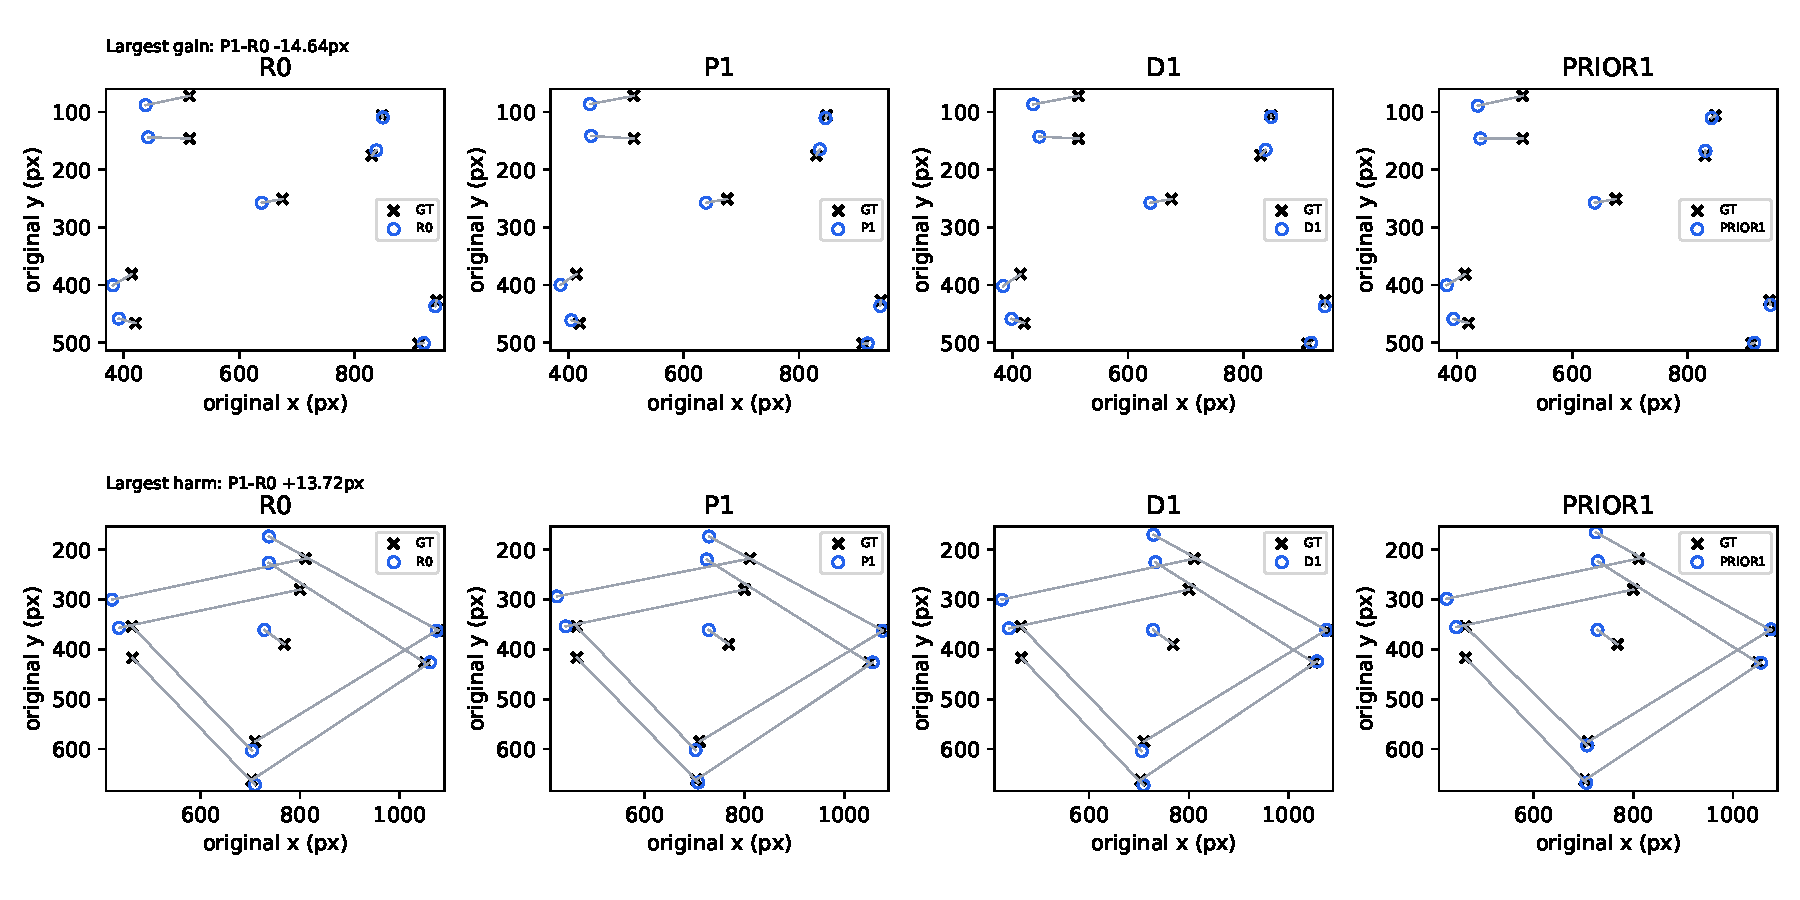
\includegraphics[width=\linewidth]{figures/qualitative_coordinates.pdf}\caption{Actual improving and harming DEV cases: the lowest and highest per-frame median difference P1--R0, with lexical frame-ID ties. Same-frame GT and every plotted model use unchanged original coordinates and shared limits. Membership and raw sources are in FIGURE\_MANIFEST.json. Images are not republished without verified image rights; these coordinate-only panels do not establish physical boundary correctness or independent generalization.}\end{figure}
P and D share source order, feature evidence and historical optimizer/exposure settings, but their loss and output geometry differ. D's small fixed-probe decrease is neither a convergence guarantee nor evidence of fundamental regression inferiority. The prior uses ImageNet TF-Slim ResNet152 initialization and the official loss/Adam semantics adapted to nine pallet points. Its sample order is exactly the existing P order and its nominal batch is sixteen. Source train/cal probes at step0 and every500 updates are diagnostic only. No checkpoint or wrapper is selected on DEV.
\begin{figure}[h]\centering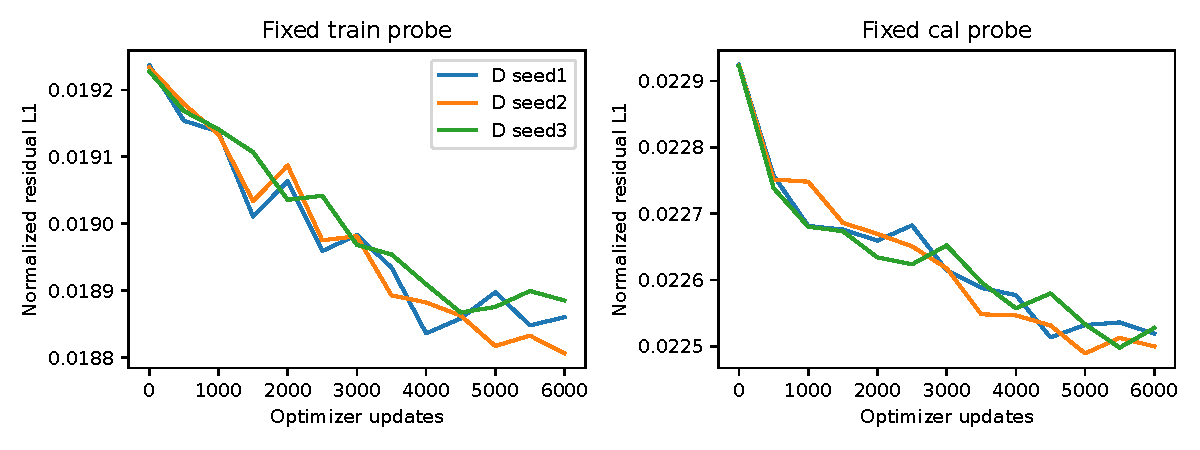
\includegraphics[width=.82\linewidth]{figures/D_probes.pdf}\caption{Already-completed D fixed probes. Their limited change is disclosed alongside the comparison, not suppressed. Loss magnitudes are not compared with P's different objective.}\end{figure}
\IfFileExists{figures/prior_probes.pdf}{\begin{figure}[h]\centering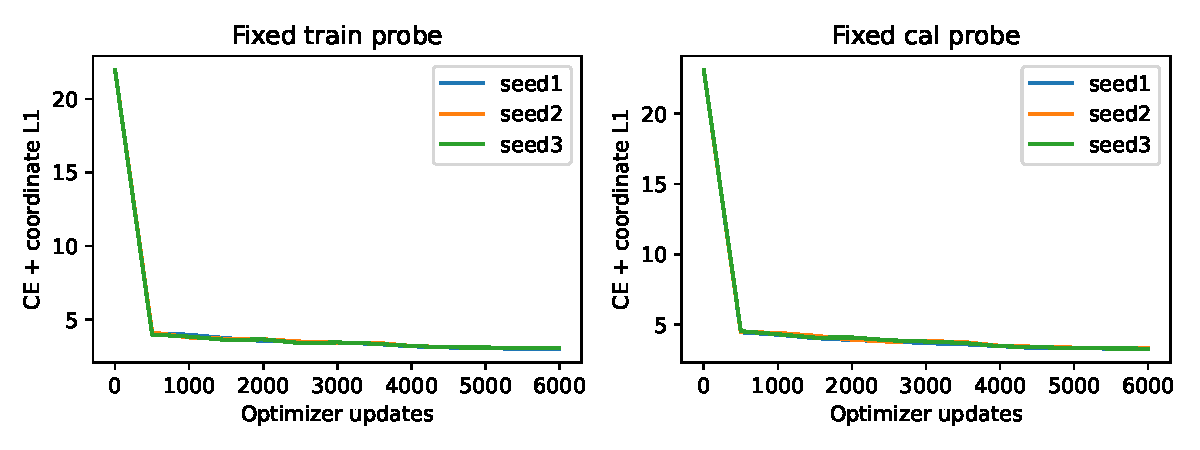
\includegraphics[width=.82\linewidth]{figures/prior_probes.pdf}\caption{Prior fixed train/cal probes from the completed bounded fits. These curves did not select a checkpoint or extend training.}\end{figure}}{}
\section{Operator and weight provenance}
The official PoseFix source commit is \texttt{5556364bb0f43b0743a5fcd820de48f34b3d4360}. Its MIT notice and the TensorFlow authors' Apache-2.0 attribution are retained. The official TF1 CPU reference runs in an isolated Python3.7 environment, and the PyTorch port uses the existing YOLO runtime without replacing that environment's Torch, CUDA, or NumPy.

The reference initializes new weights using the official graph and transfers ImageNet RGB/backbone variables. Added pose channels remain at the official seeded initialization. The port maps convolution HWIO to OIHW, transpose convolution HWOI to IOHW, and every BN affine/moving variable. Missing and unexpected keys are explicitly checked. Full eval-coordinate and stage-feature comparisons use the actual source images and the same weights; scalar/loss-gradient and moving-statistics comparisons separately test training operators.

The graph's nominal BN epsilon is not its effective value: the TF1 fused wrapper enforces $1.001\times10^{-5}$. The torch port matches this executed behavior. The Gaussian amplitude is255 exactly once. Expectation coordinates are zero-based and scaled by4 at the locked resolution. Bilinear target neighbors outside the grid are excluded and remaining mass normalized; nonfinite/outside-crop targets are masked in training, without altering evaluation membership. Raw RGB is explicitly the requested adaptation from the inspected BGR-preserving source loader.

The full batch 16 resource probe and actual parameter update are recorded separately from the three main fits. Main initialization and optimizer state do not reuse that smoke update. Checkpoints contain optimizer, Python/NumPy/CPU/CUDA RNG, step and exact order-prefix hash. The loader has no hidden random augmentation state; pending RGB reads can be reconstructed deterministically from the next recorded row.
\section{Research history and interpretation}
Prior Hough/line, active-adaptation, replay and robustness investigations motivated subsequent decisions, but do not become additional unseen validation sets. Old code, checkpoints, metrics and verdicts remain unchanged. This selection history means DEV is reused development evidence. The fixed model is not redesigned in response to an unfavorable prior comparison.

The baseline checkpoint is not purely synthetic-from-scratch: the recorded initialization checkpoint identifies COCO-pose training, despite a historical output directory containing the word scratch. P's additional training uses synthetic labels only. ImageNet supervision for the added prior is separately disclosed. These distinctions prevent an overbroad claim that no real annotation contributed anywhere.
\section{Independent data and annotation handoff}
The actual collection and schema are in \texttt{HUMAN\_INPUTS\_REQUIRED.txt} and \texttt{CONFIRMATION\_SCHEMA.json}. The starting plan is12 separate sessions with15 prespecified frames each; at least30 frames receive two independent prediction-blinded annotations and blind adjudication. The count is not a power guarantee. Preserve original videos, timestamps, capture groups, camera/mount, calibration, actual object dimensions/identity and prior-use declarations. Changed image encoding or filename does not prove independence from an old scene.

Unreviewed provenance and an unfrozen comparator panel block confirmation only, not the completed development experiment. New-frame reference geometry must be bound to its camera/dimensions/index convention before a 6D claim. Human annotation, author identities, funding and consent cannot be fabricated by the CLI. These obligations are separate from compilation and code checks.
\section{Three-estimator scope and outstanding evidence}
\ThirdEstimatorStatus{}
The third-estimator implementation and receipt-backed status are described below. No accuracy or latency is inferred from an implemented interface or a CPU input check.

\section{DOPE extension: frozen interface and training lineage}
\DopeMainStatus{}
The frozen checkpoint is \path{weights/backbone_dope_final_v1/run/final_net_epoch_0060.pth}; its SHA-256 begins \path{0de80490cb3b4f9b}, with the full digest in the protocol. The actual original training loop includes epochs 0 through 60. Original DOPE training uses random crop 400 and its recorded rotation, color, noise, and Torch FP32 normalization. The fixed inference adapter instead follows the existing reflect100--resizeback--short400 path with its existing NumPy-to-FP32 normalization. A historical header value of 448 does not describe the executed crop. No equal-baseline-epoch or identical-training/inference-normalization claim is made.

The new adapter takes BGR input and returns explicit composed affine matrices, native/canvas/network sizes, semantic point validity, hull and confidence. Taps are post-ReLU 17/26; layer 16 alone is a convolution, not the feature used. Anisotropic inverse restoration adds the transformed displacement to the retained FP64 original point. This keeps a zero move exactly equal to the baseline and prevents a fresh FP32 reprojection from introducing approximately $10^{-5}$-pixel roundoff. Fixed image-size, corner-index, GT-padding, camera and dimension contracts are required before scoring; there is no silent ID or geometry fallback.

The added P and D heads share 256/stride4 and 128/stride 8 evidence, 16-channel projections and 24 encoded channels. The backbone is in evaluation mode with gradients disabled. Newly initialized heads alone are optimized; an existing YOLO head is not a warm start. The source protocol fixes three seeds, 6,000 updates per head, batch 16 and six final fits. The AdamW learning rate is $10^{-3}$, weight decay $10^{-4}$, betas $(0.9,0.999)$, warmup 100, cosine terminal fraction 0.1, and gradient clip 5. These are head budgets, not convergence certificates for either family or equality of baseline-training cost.

Source prediction metadata is cached over the fixed source manifest; large full-resolution feature maps are not retained as a training cache. Online frozen VGG feature extraction therefore contributes actual training cost. Exact source image identities, usable rows, per-seed order hashes, final checkpoints, calibration temperatures and selected movement rules belong to the new receipts. The source mask can differ from the historical 55,915 usable YOLO rows. Nominal exposures must not be confused with successfully supervised corners; supported-frame loss reductions are retained.

\section{DOPE results, missingness and paired uncertainty}
\begin{table}[t]\centering\small
\caption{DOPE per-seed values; keypoint errors are pixels. Matched frames and pose fits have denominator319; used/excluded GT sum to2818. Excluded GT includes finite predictions on unmatched or incomplete frames, not only absent points. No failed population row is removed.}\label{tab:dopefull}
\begin{tabular}{lrrrrrrrrr}\toprule
Arm & Med. & P90 & Match & Used GT & Excl. GT & PCK10\% & Pose n & T cm & R deg\\\midrule
DOPE & 12.585 & 50.609 & 190 & 1710 & 1108 & 19.872 & 210 & 10.046 & 3.441\\
D1 & 7.857 & 47.334 & 190 & 1710 & 1108 & 35.983 & 210 & 8.352 & 2.920\\
D2 & 7.840 & 49.298 & 190 & 1710 & 1108 & 36.125 & 210 & 8.317 & 3.020\\
D3 & 7.903 & 48.831 & 190 & 1710 & 1108 & 36.054 & 210 & 8.300 & 3.115\\
P1 & 7.431 & 50.925 & 190 & 1710 & 1108 & 36.338 & 210 & 8.311 & 2.889\\
P2 & 7.422 & 50.433 & 190 & 1710 & 1108 & 37.048 & 210 & 8.496 & 2.893\\
P3 & 7.531 & 50.782 & 190 & 1710 & 1108 & 36.941 & 210 & 8.781 & 2.869\\
\bottomrule\end{tabular}
\end{table}

\begin{table*}[t]\centering\small
\caption{DOPE paired session-bootstrap differences: first arm minus second. Negative values favor the first arm for these errors. An unavailable interval denotes incompatible or empty support, not a zero effect. These reused-DEV secondary intervals are unadjusted and exploratory.}\label{tab:dopepaired}
\begin{tabular}{lrrr}\toprule
Contrast & Keypoint px [95\% CI] & T cm [95\% CI] & R deg [95\% CI]\\\midrule
P--DOPE & -5.124 [-6.304, -3.984] & -1.517 [-3.181, -0.407] & -0.558 [-1.082, -0.134]\\
D--DOPE & -4.718 [-6.035, -3.548] & -1.723 [-2.761, -0.856] & -0.423 [-1.082, -0.054]\\
P--D & -0.405 [-0.734, -0.061] & 0.206 [-1.275, 1.062] & -0.135 [-0.566, 0.221]\\
\bottomrule\end{tabular}
\end{table*}

The completed DOPE fits use 44063 usable training rows, 22034 learned parameters for P and 22522 for D. Six final fits each complete6000 updates with96000 nominal source exposures; no real images train these heads. P selects $\lambda=1.0000$ and original-image-diagonal cap none. D selects $\lambda=1.0000$ and original-image-diagonal cap none. P temperatures for seeds1--3 are 1.00, 1.00, 1.00.
\begin{table*}[t]\centering\small
\caption{DOPE source heldout partition after wrapper freezing (1985 records). This source diagnostic uses its declared partial-point support and is not the complete-nine-point DEV statistic or independent TEST.}\label{tab:dopesource}
\begin{tabular}{lrrrrr}\toprule
Arm & Med. px & P90 px & PCK10\% & Used GT & Miss GT\\\midrule
DOPE & 10.635 & 20.471 & 33.200 & 13167 & 4523\\
D1 & 4.558 & 16.948 & 57.614 & 13167 & 4523\\
D2 & 4.559 & 16.921 & 57.631 & 13167 & 4523\\
D3 & 4.560 & 16.894 & 57.513 & 13167 & 4523\\
P1 & 4.686 & 17.827 & 56.326 & 13167 & 4523\\
P2 & 4.693 & 17.886 & 56.490 & 13167 & 4523\\
P3 & 4.678 & 17.645 & 56.427 & 13167 & 4523\\
\bottomrule\end{tabular}
\end{table*}

The seven fixed arms are baseline DOPE and D1--D3/P1--P3. The complete population contains 319 positive images, 13 sessions and 2818 supervised keypoints. Every arm retains every population row, including failed or incomplete predictions. The conditional nine-point statistic requires the original box-IoU match and a finite nine-point prediction. Full-GT PCK counts excluded predictions as failures; separately labeled partial-point PCK is diagnostic only. No additional 2689-negative DOPE AP result is implied.

The evaluator reuses the canonical camera and dimension mapping, prediction-only choice of width or depth, and SQPnP followed by LM refinement. It does not let the reference pose choose a prediction hypothesis. Fewer than six finite corners, selector exceptions and failed PnP produce explicit failed rows. Pose medians use available fits and are always accompanied by coverage with denominator 319. A changed support prevents a conditional paired confidence interval rather than silently selecting a favorable intersection. Reference rotation/translation remain geometry-derived, with no new physical metrology.

Paired session and frame bootstrap reuse the existing seed 20260914 and 10000 draws. The family statistic averages per-seed pooled statistics, not predictions, and compares with one baseline. Source-selected wrappers do not use real outcomes, but the decision to run this second-estimator study followed earlier research on the same DEV population. The intervals are therefore exploratory and unadjusted. No independent TEST exists in this extension.

\section{DOPE runtime and publication records}
\begin{table*}[t]\centering\small
\caption{Measured DOPE seed-1 desktop panel, 26 prespecified images with five repeats per arm after20 warmups. Decoded RGB through real preprocessing/inference and canonical PnP; disk reads, loading and replay checks excluded. Each column is its own statistic: medians must not be added. All failure timings remain. This is a separate session from historical YOLO timing.}\label{tab:doperuntime}
\begin{tabular}{lrrrrr}\toprule
Arm & 2D med. ms & PnP med. ms & Full med. ms & Full P90 ms & Pose OK/130\\\midrule
DOPE & 60.786 & 1.625 & 62.205 & 73.310 & 85\\
DOPE+D1 & 63.888 & 1.671 & 65.038 & 76.349 & 85\\
DOPE+P1 & 63.361 & 1.678 & 64.924 & 76.220 & 85\\
\bottomrule\end{tabular}
\end{table*}
The completed panel contains 390 measured calls; coordinate replay passed at the declared absolute tolerance of 0.000000000100 pixels. Earlier failed attempts, if any, remain separately recorded and are not mixed into this completed summary. This runtime result does not establish accuracy or embedded-device throughput.

The new timing protocol records full DOPE+head RGB computation; no cached intermediate substitutes for the measured inference path. Seed 1 represents deployment without selecting the fastest seed. Keypoint and PnP-inclusive timings remain separate, and unavailable poses stay visible. Different timing sessions are not described as the historical thirteen-model session. Actual runtime receipts are needed before making any overhead or total-cost claim for DOPE.

The new experiment scripts are under \path{scripts/research/pallet_dope_refiner_20261001_v1}; the numerical records are under the matching \path{_docs/experiments/pallet_dope_refiner_20261001_v1} directory. The manuscript update script checks input bindings, population, arms and explicit completion before inserting results. \path{DOPE_RESULTS_BINDINGS.json} identifies inserted evidence, and \path{HISTORICAL_ASSETS.json} binds copied original manuscript assets. Pending evidence is stated explicitly rather than replaced by historical YOLO measurements. Build receipts certify typesetting only, not independent experimental verification or author approval.

\section{ResNet18 application: implementation and measured status}
\ResnetMainStatus{}
The third estimator is explicitly a SimpleBaseline-derived ResNet18 full-image pallet9 adaptation, not PVNet, PoseFix or a renamed DOPE stage. The ImageNet file is \path{resnet18-f37072fd.pth}, with full SHA-256 recorded in the baseline protocol. All learned body tensors and running statistics must match. The official legacy file lacks all 20 BN batch counters; the loader initializes only that complete missing counter set to zero, as in torchvision's legacy migration. Partial missing counters or missing learned tensors/running statistics stop loading. The three deconvolution layers and nine-channel head receive fresh initialization.

The $384\times512$ RGB input uses existing source reflect100 or one native-real reflection, aspect fit and centered BGR128 letterbox, followed by ImageNet FP32 normalization. No predicted or GT box is used to crop the baseline input. Actual per-axis rounded scales and inverse matrices are retained. Nine $96\times128$ Gaussian heatmaps use continuous point/4 centers, sigma 2 and square 3-sigma truncation. Source visibility greater than zero, finite non-sentinel coordinates and in-grid centers define supervision. Invalid channels remain in the fixed-nine denominator; all-masked frames remain in the batch denominator. The per-frame visibility, finite, outside-support, supervised and all-masked counts are recorded, rather than treating a low loss from absent targets as accuracy.

The specified 60-epoch baseline performs 3498 full 16-image updates plus one 12-image update each epoch, giving 3499 updates per epoch and 209940 total. The source order is a deterministic per-epoch permutation; physical batch 16 is the specified default, without a silent memory fallback. Brightness, contrast and saturation factors are independently drawn per image from $[0.8,1.2]$ in that fixed order. There is no geometric augmentation. Model and target arithmetic are FP32 with AMP and TF32 disabled. Adam uses betas $(0.9,0.999)$, learning rate $0.001$, weight decay $0.0001$, with drops at the beginning of epochs 40 and 50. No real score chooses the schedule, threshold, stopping epoch or checkpoint.

Epoch loss is weighted by actual frame counts, including the final 12-frame batch. Training supervision counts cover 60 epochs of exposures rather than unique images. The calibration 1004 loss and full mask counts are recorded without PnP, heldout or real accuracy selection. Checkpoints carry the in-progress epoch numerator/frame count and cumulative mask counts, so an infrastructure resume does not double-count them. Private DataLoader generators isolate the saved model/augmentation RNG stream; final export can be completed after interruption without replacing a verified final model. The prescribed eight-update GPU smoke is discarded and excluded from the main budget; no smoke speed or learned accuracy is reported here.

After the independently trained baseline is frozen, its layer2 and layer3 outputs give 128 channels at stride 8 and 256 at stride 16. New P/D heads use the unchanged local evidence and source-selection principles for three seeds and 6000 updates of 16 examples per head. The trained baseline checkpoint, baseline protocol and baseline-completion SHA are required before that second protocol can be created. An ImageNet-only network is never silently used as the trained pallet baseline. \ResnetBaselineStatus{}

\section{ResNet18 results and cost}
\begin{table}[t]\centering\small
\caption{Primary ResNet18 arm by seed on reused DEV319. FULL is one frozen baseline; all rows preserve its 299 matched frames and 319/319 pose coverage. R is the canonical MAIN camera-facing-frame C2 rotation.}\label{tab:resnetfull}
\begin{tabular}{lrrrrr}\toprule
Arm & Med. px & P90 px & PCK10\% & T cm & R-C2 deg\\\midrule
FULL & 8.001 & 52.054 & 54.68 & 11.007 & 3.252\\
D0-S1 & 7.868 & 52.065 & 55.18 & 9.784 & 3.283\\
D0-S2 & 7.809 & 51.823 & 55.46 & 9.927 & 3.145\\
D0-S3 & 7.880 & 51.897 & 55.15 & 9.798 & 3.227\\
P0-S1 & 7.141 & 51.923 & 58.23 & 9.963 & 3.009\\
P0-S2 & 7.157 & 52.198 & 58.16 & 9.884 & 3.052\\
P0-S3 & 7.129 & 52.139 & 58.45 & 10.154 & 2.994\\
\bottomrule\end{tabular}
\end{table}

\begin{table*}[t]\centering\footnotesize
\caption{Primary ResNet18 paired session-bootstrap differences on reused DEV: head minus FULL. Negative favors the head for 2D/T/R; positive favors it for PCK10. Intervals use 10,000 session resamples and are exploratory, unadjusted, and do not create an independent test.}\label{tab:resnetpaired}
\begin{tabular}{lrrrr}\toprule
Contrast & 2D change px [95\% CI] & PCK10 change pp [95\% CI] & T change cm [95\% CI] & R-C2 change deg [95\% CI]\\\midrule
D0--FULL & -0.149 [-0.316,-0.048] & 0.580 [0.242,0.983] & -1.171 [-1.388,0.149] & -0.034 [-0.216,0.062]\\
P0--FULL & -0.859 [-1.318,-0.621] & 3.596 [2.515,4.986] & -1.007 [-1.668,0.187] & -0.234 [-0.502,-0.022]\\
\bottomrule\end{tabular}
\end{table*}

The frozen FULL baseline yields 55,804 usable synthetic TRAIN rows. D0, P0, P5 and P5\_CONSTANT each use three seeds of 6,000 AdamW updates at batch 16 (96,000 nominal exposures per fit) and zero real training images. Trainable counts are 22,522 for D0, 22,034 for P0, and 23,331 for each P5 arm. Synthetic selection fixes $\lambda=1$ for every arm, a 0.01 image-diagonal cap only for D0, no cap for P0/P5, and temperature 1 for all probability heads.
\begin{table}[t]\centering\small
\caption{Frozen synthetic heldout diagnostic after source-only rule selection (1,985 records). Head rows are means of three seed statistics; this reused source partition is not an independent real-image test.}\label{tab:resnetsource}
\begin{tabular}{lrrr}\toprule
Arm & Med. px & P90 px & PCK10\%\\\midrule
FULL & 2.805 & 9.499 & 89.723\\
D0 mean & 2.694 & 9.504 & 89.721\\
P0 mean & 2.585 & 9.510 & 89.710\\
P5 mean & 2.585 & 9.500 & 89.674\\
P5\_CONSTANT mean & 2.585 & 9.506 & 89.674\\
\bottomrule\end{tabular}
\end{table}

ResNet18 baseline completion and its full 60-epoch training/calibration loss curve remain pending. No simulated curve is shown.

\begin{table}[t]\centering\small
\caption{Integrated desktop timing for the ResNet18 arms. Each arm uses the same 26 decoded BGR images, 20 warmups, batch one, five repeats, and seed 1 for a learned head. PnP and full columns are separately summarized; their medians are not arithmetically additive.}\label{tab:resnetruntime}
\begin{tabular}{lrrrr}\toprule
Arm & 2D med. & 2D P90 & Full med. & Full P90\\\midrule
FULL & 7.835 & 10.432 & 9.453 & 12.146\\
D0-S1 & 10.104 & 13.410 & 11.886 & 14.838\\
P0-S1 & 10.520 & 13.565 & 12.193 & 14.982\\
P5-C-S1 & 11.442 & 13.790 & 13.132 & 15.228\\
P5-S1 & 11.302 & 13.977 & 12.963 & 15.342\\
\bottomrule\end{tabular}
\end{table}

These results reuse DEV and the geometry-derived reference; completion of three fixed applications does not create independent TEST or a physical T/R stability guarantee. The ResNet18 insertion record is \path{RESNET_RESULTS_BINDINGS.json}.

\section{Reproduction and access}
From the repository root, use the recorded environment and \texttt{run.py status}, \texttt{run.py all}, or \texttt{run.py resume} under \texttt{scripts/research/pallet\_sensors\_submission\_v1/}. Exact shell commands, downloads, locks and stage receipts are in \texttt{REPRODUCE.md}. Completion receipts are checked against actual input/output hashes, not accepted solely on a status string. Main uses no branch rewrite, force push or deletion of unrelated user changes.

Public materials contain code, small numerical results, plots and manuscript sources. Raw training/evaluation imagery, video, feature caches, model weights and the isolated environment remain excluded from public Git. Access restrictions and licenses must be reviewed before any separate sharing. No unverified speedup, annotation-cost reduction, or public-data right is inferred.
\end{document}
